% Options for packages loaded elsewhere
\PassOptionsToPackage{unicode}{hyperref}
\PassOptionsToPackage{hyphens}{url}
\PassOptionsToPackage{dvipsnames,svgnames,x11names}{xcolor}
%
\documentclass[
  letterpaper,
  DIV=11,
  numbers=noendperiod]{scrreprt}
\usepackage{amsmath,amssymb}
\usepackage{lmodern}
\usepackage{iftex}
\ifPDFTeX
  \usepackage[T1]{fontenc}
  \usepackage[utf8]{inputenc}
  \usepackage{textcomp} % provide euro and other symbols
\else % if luatex or xetex
  \usepackage{unicode-math}
  \defaultfontfeatures{Scale=MatchLowercase}
  \defaultfontfeatures[\rmfamily]{Ligatures=TeX,Scale=1}
\fi
% Use upquote if available, for straight quotes in verbatim environments
\IfFileExists{upquote.sty}{\usepackage{upquote}}{}
\IfFileExists{microtype.sty}{% use microtype if available
  \usepackage[]{microtype}
  \UseMicrotypeSet[protrusion]{basicmath} % disable protrusion for tt fonts
}{}
\makeatletter
\@ifundefined{KOMAClassName}{% if non-KOMA class
  \IfFileExists{parskip.sty}{%
    \usepackage{parskip}
  }{% else
    \setlength{\parindent}{0pt}
    \setlength{\parskip}{6pt plus 2pt minus 1pt}}
}{% if KOMA class
  \KOMAoptions{parskip=half}}
\makeatother
\usepackage{xcolor}
\setlength{\emergencystretch}{3em} % prevent overfull lines
\setcounter{secnumdepth}{5}
% Make \paragraph and \subparagraph free-standing
\ifx\paragraph\undefined\else
  \let\oldparagraph\paragraph
  \renewcommand{\paragraph}[1]{\oldparagraph{#1}\mbox{}}
\fi
\ifx\subparagraph\undefined\else
  \let\oldsubparagraph\subparagraph
  \renewcommand{\subparagraph}[1]{\oldsubparagraph{#1}\mbox{}}
\fi

\usepackage{color}
\usepackage{fancyvrb}
\newcommand{\VerbBar}{|}
\newcommand{\VERB}{\Verb[commandchars=\\\{\}]}
\DefineVerbatimEnvironment{Highlighting}{Verbatim}{commandchars=\\\{\}}
% Add ',fontsize=\small' for more characters per line
\usepackage{framed}
\definecolor{shadecolor}{RGB}{241,243,245}
\newenvironment{Shaded}{\begin{snugshade}}{\end{snugshade}}
\newcommand{\AlertTok}[1]{\textcolor[rgb]{0.68,0.00,0.00}{#1}}
\newcommand{\AnnotationTok}[1]{\textcolor[rgb]{0.37,0.37,0.37}{#1}}
\newcommand{\AttributeTok}[1]{\textcolor[rgb]{0.40,0.45,0.13}{#1}}
\newcommand{\BaseNTok}[1]{\textcolor[rgb]{0.68,0.00,0.00}{#1}}
\newcommand{\BuiltInTok}[1]{\textcolor[rgb]{0.00,0.23,0.31}{#1}}
\newcommand{\CharTok}[1]{\textcolor[rgb]{0.13,0.47,0.30}{#1}}
\newcommand{\CommentTok}[1]{\textcolor[rgb]{0.37,0.37,0.37}{#1}}
\newcommand{\CommentVarTok}[1]{\textcolor[rgb]{0.37,0.37,0.37}{\textit{#1}}}
\newcommand{\ConstantTok}[1]{\textcolor[rgb]{0.56,0.35,0.01}{#1}}
\newcommand{\ControlFlowTok}[1]{\textcolor[rgb]{0.00,0.23,0.31}{#1}}
\newcommand{\DataTypeTok}[1]{\textcolor[rgb]{0.68,0.00,0.00}{#1}}
\newcommand{\DecValTok}[1]{\textcolor[rgb]{0.68,0.00,0.00}{#1}}
\newcommand{\DocumentationTok}[1]{\textcolor[rgb]{0.37,0.37,0.37}{\textit{#1}}}
\newcommand{\ErrorTok}[1]{\textcolor[rgb]{0.68,0.00,0.00}{#1}}
\newcommand{\ExtensionTok}[1]{\textcolor[rgb]{0.00,0.23,0.31}{#1}}
\newcommand{\FloatTok}[1]{\textcolor[rgb]{0.68,0.00,0.00}{#1}}
\newcommand{\FunctionTok}[1]{\textcolor[rgb]{0.28,0.35,0.67}{#1}}
\newcommand{\ImportTok}[1]{\textcolor[rgb]{0.00,0.46,0.62}{#1}}
\newcommand{\InformationTok}[1]{\textcolor[rgb]{0.37,0.37,0.37}{#1}}
\newcommand{\KeywordTok}[1]{\textcolor[rgb]{0.00,0.23,0.31}{#1}}
\newcommand{\NormalTok}[1]{\textcolor[rgb]{0.00,0.23,0.31}{#1}}
\newcommand{\OperatorTok}[1]{\textcolor[rgb]{0.37,0.37,0.37}{#1}}
\newcommand{\OtherTok}[1]{\textcolor[rgb]{0.00,0.23,0.31}{#1}}
\newcommand{\PreprocessorTok}[1]{\textcolor[rgb]{0.68,0.00,0.00}{#1}}
\newcommand{\RegionMarkerTok}[1]{\textcolor[rgb]{0.00,0.23,0.31}{#1}}
\newcommand{\SpecialCharTok}[1]{\textcolor[rgb]{0.37,0.37,0.37}{#1}}
\newcommand{\SpecialStringTok}[1]{\textcolor[rgb]{0.13,0.47,0.30}{#1}}
\newcommand{\StringTok}[1]{\textcolor[rgb]{0.13,0.47,0.30}{#1}}
\newcommand{\VariableTok}[1]{\textcolor[rgb]{0.07,0.07,0.07}{#1}}
\newcommand{\VerbatimStringTok}[1]{\textcolor[rgb]{0.13,0.47,0.30}{#1}}
\newcommand{\WarningTok}[1]{\textcolor[rgb]{0.37,0.37,0.37}{\textit{#1}}}

\providecommand{\tightlist}{%
  \setlength{\itemsep}{0pt}\setlength{\parskip}{0pt}}\usepackage{longtable,booktabs,array}
\usepackage{calc} % for calculating minipage widths
% Correct order of tables after \paragraph or \subparagraph
\usepackage{etoolbox}
\makeatletter
\patchcmd\longtable{\par}{\if@noskipsec\mbox{}\fi\par}{}{}
\makeatother
% Allow footnotes in longtable head/foot
\IfFileExists{footnotehyper.sty}{\usepackage{footnotehyper}}{\usepackage{footnote}}
\makesavenoteenv{longtable}
\usepackage{graphicx}
\makeatletter
\def\maxwidth{\ifdim\Gin@nat@width>\linewidth\linewidth\else\Gin@nat@width\fi}
\def\maxheight{\ifdim\Gin@nat@height>\textheight\textheight\else\Gin@nat@height\fi}
\makeatother
% Scale images if necessary, so that they will not overflow the page
% margins by default, and it is still possible to overwrite the defaults
% using explicit options in \includegraphics[width, height, ...]{}
\setkeys{Gin}{width=\maxwidth,height=\maxheight,keepaspectratio}
% Set default figure placement to htbp
\makeatletter
\def\fps@figure{htbp}
\makeatother
\newlength{\cslhangindent}
\setlength{\cslhangindent}{1.5em}
\newlength{\csllabelwidth}
\setlength{\csllabelwidth}{3em}
\newlength{\cslentryspacingunit} % times entry-spacing
\setlength{\cslentryspacingunit}{\parskip}
\newenvironment{CSLReferences}[2] % #1 hanging-ident, #2 entry spacing
 {% don't indent paragraphs
  \setlength{\parindent}{0pt}
  % turn on hanging indent if param 1 is 1
  \ifodd #1
  \let\oldpar\par
  \def\par{\hangindent=\cslhangindent\oldpar}
  \fi
  % set entry spacing
  \setlength{\parskip}{#2\cslentryspacingunit}
 }%
 {}
\usepackage{calc}
\newcommand{\CSLBlock}[1]{#1\hfill\break}
\newcommand{\CSLLeftMargin}[1]{\parbox[t]{\csllabelwidth}{#1}}
\newcommand{\CSLRightInline}[1]{\parbox[t]{\linewidth - \csllabelwidth}{#1}\break}
\newcommand{\CSLIndent}[1]{\hspace{\cslhangindent}#1}

\KOMAoption{captions}{tableheading}
\makeatletter
\makeatother
\makeatletter
\@ifpackageloaded{caption}{}{\usepackage{caption}}
\AtBeginDocument{%
\ifdefined\contentsname
  \renewcommand*\contentsname{Table of contents}
\else
  \newcommand\contentsname{Table of contents}
\fi
\ifdefined\listfigurename
  \renewcommand*\listfigurename{List of Figures}
\else
  \newcommand\listfigurename{List of Figures}
\fi
\ifdefined\listtablename
  \renewcommand*\listtablename{List of Tables}
\else
  \newcommand\listtablename{List of Tables}
\fi
\ifdefined\figurename
  \renewcommand*\figurename{Figure}
\else
  \newcommand\figurename{Figure}
\fi
\ifdefined\tablename
  \renewcommand*\tablename{Table}
\else
  \newcommand\tablename{Table}
\fi
}
\@ifpackageloaded{float}{}{\usepackage{float}}
\floatstyle{ruled}
\@ifundefined{c@chapter}{\newfloat{codelisting}{h}{lop}}{\newfloat{codelisting}{h}{lop}[chapter]}
\floatname{codelisting}{Listing}
\newcommand*\listoflistings{\listof{codelisting}{List of Listings}}
\makeatother
\makeatletter
\@ifpackageloaded{caption}{}{\usepackage{caption}}
\@ifpackageloaded{subcaption}{}{\usepackage{subcaption}}
\makeatother
\makeatletter
\@ifpackageloaded{tcolorbox}{}{\usepackage[many]{tcolorbox}}
\makeatother
\makeatletter
\@ifundefined{shadecolor}{\definecolor{shadecolor}{rgb}{.97, .97, .97}}
\makeatother
\makeatletter
\makeatother
\ifLuaTeX
  \usepackage{selnolig}  % disable illegal ligatures
\fi
\IfFileExists{bookmark.sty}{\usepackage{bookmark}}{\usepackage{hyperref}}
\IfFileExists{xurl.sty}{\usepackage{xurl}}{} % add URL line breaks if available
\urlstyle{same} % disable monospaced font for URLs
\hypersetup{
  pdftitle={gcs\_jps},
  pdfauthor={Greta Timaite},
  colorlinks=true,
  linkcolor={blue},
  filecolor={Maroon},
  citecolor={Blue},
  urlcolor={Blue},
  pdfcreator={LaTeX via pandoc}}

\title{gcs\_jps}
\author{Greta Timaite}
\date{9/5/2022}

\begin{document}
\maketitle

\ifdefined\Shaded\renewenvironment{Shaded}{\begin{tcolorbox}[sharp corners, breakable, interior hidden, frame hidden, boxrule=0pt, enhanced, borderline west={3pt}{0pt}{shadecolor}]}{\end{tcolorbox}}\fi

\renewcommand*\contentsname{Table of contents}
{
\hypersetup{linkcolor=}
\setcounter{tocdepth}{2}
\tableofcontents
}
\hypertarget{preface}{%
\chapter*{Preface}\label{preface}}
\addcontentsline{toc}{chapter}{Preface}

This is a Quarto book.

To learn more about Quarto books visit
\url{https://quarto.org/docs/books}.

\begin{Shaded}
\begin{Highlighting}[]
\DecValTok{1} \SpecialCharTok{+} \DecValTok{1}
\end{Highlighting}
\end{Shaded}

\begin{verbatim}
[1] 2
\end{verbatim}

\hypertarget{getting-data}{%
\chapter{Getting data}\label{getting-data}}

\begin{Shaded}
\begin{Highlighting}[]
\CommentTok{\# trajectory data}
\NormalTok{traj1 }\OtherTok{=} \FunctionTok{read.table}\NormalTok{(}\StringTok{"/Users/gretatimaite/Desktop/pedestrian\_simulation/final\_results/8\_frame/1/traj.txt"}\NormalTok{,}
                   \AttributeTok{col.names =} \FunctionTok{c}\NormalTok{(}\StringTok{"ID"}\NormalTok{,  }\StringTok{"FR"}\NormalTok{,   }\StringTok{"X"}\NormalTok{,    }\StringTok{"Y"}\NormalTok{,    }\StringTok{"Z"}\NormalTok{,    }\StringTok{"A"}\NormalTok{,    }\StringTok{"B"}\NormalTok{,    }\StringTok{"ANGLE"}\NormalTok{,    }\StringTok{"COLOR"}\NormalTok{))}

\NormalTok{traj1 }\SpecialCharTok{|\textgreater{}}\NormalTok{ dplyr}\SpecialCharTok{::}\FunctionTok{glimpse}\NormalTok{()}
\end{Highlighting}
\end{Shaded}

\begin{verbatim}
Rows: 169,605
Columns: 9
$ ID    <int> 284, 285, 286, 287, 288, 289, 290, 291, 292, 293, 294, 295, 296,~
$ FR    <int> 0, 0, 0, 0, 0, 0, 0, 0, 0, 0, 0, 0, 0, 0, 0, 0, 0, 0, 0, 0, 0, 0~
$ X     <dbl> 3.75, 2.50, 2.50, 2.50, 2.50, 9.00, 13.84, 16.67, 15.26, 16.67, ~
$ Y     <dbl> 20.00, 25.23, 14.77, 28.27, 11.72, 47.50, 47.50, 47.50, 45.14, 4~
$ Z     <dbl> 0, 0, 0, 0, 0, 0, 0, 0, 0, 0, 0, 0, 0, 0, 0, 0, 0, 0, 0, 0, 0, 0~
$ A     <dbl> 0.15, 0.15, 0.15, 0.15, 0.15, 0.15, 0.15, 0.15, 0.15, 0.15, 0.15~
$ B     <dbl> 0.15, 0.15, 0.15, 0.15, 0.15, 0.15, 0.15, 0.15, 0.15, 0.15, 0.15~
$ ANGLE <dbl> 90.00, 40.01, 16.79, -3.71, -26.03, -117.22, -12.25, -31.77, -61~
$ COLOR <int> 0, 0, 0, 0, 0, 0, 0, 0, 0, 0, 0, 0, 0, 0, 0, 0, 0, 0, 0, 0, 0, 0~
\end{verbatim}

\begin{Shaded}
\begin{Highlighting}[]
\CommentTok{\# clean GCS data}

\NormalTok{gcs }\OtherTok{=}\NormalTok{ sf}\SpecialCharTok{::}\FunctionTok{read\_sf}\NormalTok{(}\StringTok{"https://github.com/GretaTimaite/pedestrian\_simulation/releases/download/data/frames\_final.csv"}\NormalTok{)}
\end{Highlighting}
\end{Shaded}

\begin{Shaded}
\begin{Highlighting}[]
\CommentTok{\# let\textquotesingle{}s convert jps and gcs dataframes to sf objects, so we can perform spatial operations}

\NormalTok{traj1\_sf }\OtherTok{=}\NormalTok{ traj1 }\SpecialCharTok{|\textgreater{}} 
\NormalTok{  sf}\SpecialCharTok{::}\FunctionTok{st\_as\_sf}\NormalTok{(}\AttributeTok{coords =} \FunctionTok{c}\NormalTok{(}\StringTok{"X"}\NormalTok{, }\StringTok{"Y"}\NormalTok{)) }\SpecialCharTok{|\textgreater{}} 
\NormalTok{  dplyr}\SpecialCharTok{::}\FunctionTok{select}\NormalTok{(}\SpecialCharTok{{-}}\FunctionTok{c}\NormalTok{(}\DecValTok{3}\NormalTok{,}\DecValTok{4}\NormalTok{,}\DecValTok{5}\NormalTok{,}\DecValTok{6}\NormalTok{,}\DecValTok{7}\NormalTok{)) }\CommentTok{\# drop columns we won\textquotesingle{}t need}

\NormalTok{gcs\_sf }\OtherTok{=}\NormalTok{ gcs }\SpecialCharTok{|\textgreater{}} 
\NormalTok{  sf}\SpecialCharTok{::}\FunctionTok{st\_as\_sf}\NormalTok{(}\AttributeTok{coords =} \FunctionTok{c}\NormalTok{(}\StringTok{"x\_coord"}\NormalTok{, }\StringTok{"y\_coord"}\NormalTok{)) }\SpecialCharTok{|\textgreater{}} 
\NormalTok{  dplyr}\SpecialCharTok{::}\FunctionTok{mutate}\NormalTok{(}\AttributeTok{geometry =}\NormalTok{ geometry}\SpecialCharTok{/}\DecValTok{14}\NormalTok{) }\CommentTok{\# convert from pixels to metres}
\end{Highlighting}
\end{Shaded}

\hypertarget{environment}{%
\chapter{Environment}\label{environment}}

In this section we will prepare the environment for further analysis.
Concourse parameters: width(x) = 53, height(y) = 50;

\hypertarget{global}{%
\section{Global}\label{global}}

\begin{Shaded}
\begin{Highlighting}[]
\CommentTok{\# First let\textquotesingle{}s define an area in metres}
\NormalTok{gcs\_env\_m }\OtherTok{=} \ControlFlowTok{function}\NormalTok{()\{}
  \FunctionTok{plot}\NormalTok{((}\SpecialCharTok{{-}}\DecValTok{250} \SpecialCharTok{/}\DecValTok{14}\NormalTok{)}\SpecialCharTok{:}\NormalTok{(}\DecValTok{900}\SpecialCharTok{/}\DecValTok{14}\NormalTok{), (}\SpecialCharTok{{-}}\DecValTok{250}\SpecialCharTok{/}\DecValTok{14}\NormalTok{)}\SpecialCharTok{:}\NormalTok{(}\DecValTok{900}\SpecialCharTok{/}\DecValTok{14}\NormalTok{), }\AttributeTok{col =} \StringTok{"white"}\NormalTok{, }\AttributeTok{xlab =} \StringTok{"X"}\NormalTok{, }\AttributeTok{ylab =} \StringTok{"Y"}\NormalTok{) }\CommentTok{\# draw an empty plot}
  \FunctionTok{polygon}\NormalTok{(}\AttributeTok{x =} \FunctionTok{c}\NormalTok{(}\DecValTok{0}\NormalTok{, }\DecValTok{0}\NormalTok{, }\DecValTok{740}\SpecialCharTok{/}\DecValTok{14}\NormalTok{, }\DecValTok{740}\SpecialCharTok{/}\DecValTok{14}\NormalTok{),}
          \AttributeTok{y =} \FunctionTok{c}\NormalTok{(}\DecValTok{0}\NormalTok{, }\DecValTok{700}\SpecialCharTok{/}\DecValTok{14}\NormalTok{, }\DecValTok{700}\SpecialCharTok{/}\DecValTok{14}\NormalTok{, }\DecValTok{0}\NormalTok{),}
          \AttributeTok{border =} \StringTok{"blue"}\NormalTok{,}
          \AttributeTok{lwd =} \DecValTok{2}\NormalTok{) }\CommentTok{\# draw walls of a GCS}
  \FunctionTok{polygon}\NormalTok{(}\AttributeTok{x=} \FunctionTok{c}\NormalTok{(}\SpecialCharTok{{-}}\DecValTok{150}\SpecialCharTok{/}\DecValTok{14}\NormalTok{, }\DecValTok{0}\NormalTok{, }\DecValTok{0}\NormalTok{, }\SpecialCharTok{{-}}\DecValTok{150}\SpecialCharTok{/}\DecValTok{14}\NormalTok{),}
          \AttributeTok{y =} \FunctionTok{c}\NormalTok{(}\DecValTok{400}\SpecialCharTok{/}\DecValTok{14}\NormalTok{, }\DecValTok{400}\SpecialCharTok{/}\DecValTok{14}\NormalTok{, }\DecValTok{150}\SpecialCharTok{/}\DecValTok{14}\NormalTok{, }\DecValTok{150}\SpecialCharTok{/}\DecValTok{14}\NormalTok{),}
          \AttributeTok{border =} \StringTok{"blue"}\NormalTok{,}
          \AttributeTok{lwd =} \DecValTok{2}\NormalTok{) }\CommentTok{\# exit 0}
  \FunctionTok{polygon}\NormalTok{(}\AttributeTok{x =} \FunctionTok{c}\NormalTok{(}\DecValTok{0}\NormalTok{, }\DecValTok{250}\SpecialCharTok{/}\DecValTok{14}\NormalTok{, }\DecValTok{250}\SpecialCharTok{/}\DecValTok{14}\NormalTok{, }\DecValTok{0}\NormalTok{),}
          \AttributeTok{y =} \FunctionTok{c}\NormalTok{(}\DecValTok{850}\SpecialCharTok{/}\DecValTok{14}\NormalTok{, }\DecValTok{850}\SpecialCharTok{/}\DecValTok{14}\NormalTok{, }\DecValTok{700}\SpecialCharTok{/}\DecValTok{14}\NormalTok{, }\DecValTok{700}\SpecialCharTok{/}\DecValTok{14}\NormalTok{),}
          \AttributeTok{border =} \StringTok{"red"}\NormalTok{,}
          \AttributeTok{lwd =} \DecValTok{2}\NormalTok{) }\CommentTok{\# exit 1}
  \FunctionTok{polygon}\NormalTok{(}\AttributeTok{x =} \FunctionTok{c}\NormalTok{(}\DecValTok{455}\SpecialCharTok{/}\DecValTok{14}\NormalTok{, }\DecValTok{700}\SpecialCharTok{/}\DecValTok{14}\NormalTok{, }\DecValTok{700}\SpecialCharTok{/}\DecValTok{14}\NormalTok{, }\DecValTok{455}\SpecialCharTok{/}\DecValTok{14}\NormalTok{),}
          \AttributeTok{y =} \FunctionTok{c}\NormalTok{(}\DecValTok{850}\SpecialCharTok{/}\DecValTok{14}\NormalTok{, }\DecValTok{850}\SpecialCharTok{/}\DecValTok{14}\NormalTok{, }\DecValTok{700}\SpecialCharTok{/}\DecValTok{14}\NormalTok{, }\DecValTok{700}\SpecialCharTok{/}\DecValTok{14}\NormalTok{),}
          \AttributeTok{border =} \StringTok{"red"}\NormalTok{,}
          \AttributeTok{lwd =} \DecValTok{2}\NormalTok{) }\CommentTok{\# exit 2}
  \FunctionTok{polygon}\NormalTok{(}\AttributeTok{x =} \FunctionTok{c}\NormalTok{(}\DecValTok{740}\SpecialCharTok{/}\DecValTok{14}\NormalTok{, }\DecValTok{860}\SpecialCharTok{/}\DecValTok{14}\NormalTok{, }\DecValTok{860}\SpecialCharTok{/}\DecValTok{14}\NormalTok{, }\DecValTok{740}\SpecialCharTok{/}\DecValTok{14}\NormalTok{),}
          \AttributeTok{y =} \FunctionTok{c}\NormalTok{(}\DecValTok{700}\SpecialCharTok{/}\DecValTok{14}\NormalTok{, }\DecValTok{700}\SpecialCharTok{/}\DecValTok{14}\NormalTok{, }\DecValTok{610}\SpecialCharTok{/}\DecValTok{14}\NormalTok{, }\DecValTok{610}\SpecialCharTok{/}\DecValTok{14}\NormalTok{),}
          \AttributeTok{border =} \StringTok{"red"}\NormalTok{,}
          \AttributeTok{lwd =} \DecValTok{2}\NormalTok{) }\CommentTok{\# exit 3}
  \FunctionTok{polygon}\NormalTok{(}\AttributeTok{x =} \FunctionTok{c}\NormalTok{(}\DecValTok{740}\SpecialCharTok{/}\DecValTok{14}\NormalTok{, }\DecValTok{860}\SpecialCharTok{/}\DecValTok{14}\NormalTok{, }\DecValTok{860}\SpecialCharTok{/}\DecValTok{14}\NormalTok{, }\DecValTok{740}\SpecialCharTok{/}\DecValTok{14}\NormalTok{),}
          \AttributeTok{y =} \FunctionTok{c}\NormalTok{(}\DecValTok{550}\SpecialCharTok{/}\DecValTok{14}\NormalTok{, }\DecValTok{550}\SpecialCharTok{/}\DecValTok{14}\NormalTok{, }\DecValTok{400}\SpecialCharTok{/}\DecValTok{14}\NormalTok{, }\DecValTok{400}\SpecialCharTok{/}\DecValTok{14}\NormalTok{),}
          \AttributeTok{border =} \StringTok{"red"}\NormalTok{,}
          \AttributeTok{lwd =} \DecValTok{2}\NormalTok{) }\CommentTok{\# exit 4}
  \FunctionTok{polygon}\NormalTok{(}\AttributeTok{x =} \FunctionTok{c}\NormalTok{(}\DecValTok{740}\SpecialCharTok{/}\DecValTok{14}\NormalTok{, }\DecValTok{860}\SpecialCharTok{/}\DecValTok{14}\NormalTok{, }\DecValTok{860}\SpecialCharTok{/}\DecValTok{14}\NormalTok{, }\DecValTok{740}\SpecialCharTok{/}\DecValTok{14}\NormalTok{),}
          \AttributeTok{y =} \FunctionTok{c}\NormalTok{(}\DecValTok{340}\SpecialCharTok{/}\DecValTok{14}\NormalTok{, }\DecValTok{340}\SpecialCharTok{/}\DecValTok{14}\NormalTok{, }\DecValTok{190}\SpecialCharTok{/}\DecValTok{14}\NormalTok{, }\DecValTok{190}\SpecialCharTok{/}\DecValTok{14}\NormalTok{),}
          \AttributeTok{border =} \StringTok{"red"}\NormalTok{,}
          \AttributeTok{lwd =} \DecValTok{2}\NormalTok{) }\CommentTok{\# exit 5}
  \FunctionTok{polygon}\NormalTok{(}\AttributeTok{x =} \FunctionTok{c}\NormalTok{(}\DecValTok{740}\SpecialCharTok{/}\DecValTok{14}\NormalTok{, }\DecValTok{860}\SpecialCharTok{/}\DecValTok{14}\NormalTok{, }\DecValTok{860}\SpecialCharTok{/}\DecValTok{14}\NormalTok{, }\DecValTok{740}\SpecialCharTok{/}\DecValTok{14}\NormalTok{),}
          \AttributeTok{y =} \FunctionTok{c}\NormalTok{(}\DecValTok{130}\SpecialCharTok{/}\DecValTok{14}\NormalTok{, }\DecValTok{130}\SpecialCharTok{/}\DecValTok{14}\NormalTok{, }\DecValTok{0}\NormalTok{, }\DecValTok{0}\NormalTok{),}
          \AttributeTok{border =} \StringTok{"red"}\NormalTok{,}
          \AttributeTok{lwd =} \DecValTok{2}\NormalTok{) }\CommentTok{\# exit 6}
  \FunctionTok{polygon}\NormalTok{(}\AttributeTok{x =} \FunctionTok{c}\NormalTok{(}\DecValTok{555}\SpecialCharTok{/}\DecValTok{14}\NormalTok{, }\DecValTok{740}\SpecialCharTok{/}\DecValTok{14}\NormalTok{, }\DecValTok{740}\SpecialCharTok{/}\DecValTok{14}\NormalTok{, }\DecValTok{555}\SpecialCharTok{/}\DecValTok{14}\NormalTok{),}
          \AttributeTok{y =} \FunctionTok{c}\NormalTok{(}\DecValTok{0}\NormalTok{, }\DecValTok{0}\NormalTok{, }\SpecialCharTok{{-}}\DecValTok{70}\SpecialCharTok{/}\DecValTok{14}\NormalTok{, }\SpecialCharTok{{-}}\DecValTok{70}\SpecialCharTok{/}\DecValTok{14}\NormalTok{),}
          \AttributeTok{border =} \StringTok{"red"}\NormalTok{,}
          \AttributeTok{lwd =} \DecValTok{2}\NormalTok{) }\CommentTok{\# exit 7}
  \FunctionTok{polygon}\NormalTok{(}\AttributeTok{x =} \FunctionTok{c}\NormalTok{(}\DecValTok{370}\SpecialCharTok{/}\DecValTok{14}\NormalTok{, }\DecValTok{555}\SpecialCharTok{/}\DecValTok{14}\NormalTok{, }\DecValTok{556}\SpecialCharTok{/}\DecValTok{14}\NormalTok{, }\DecValTok{370}\SpecialCharTok{/}\DecValTok{14}\NormalTok{),}
          \AttributeTok{y =} \FunctionTok{c}\NormalTok{(}\DecValTok{0}\NormalTok{, }\DecValTok{0}\NormalTok{, }\SpecialCharTok{{-}}\DecValTok{70}\SpecialCharTok{/}\DecValTok{14}\NormalTok{, }\SpecialCharTok{{-}}\DecValTok{70}\SpecialCharTok{/}\DecValTok{14}\NormalTok{),}
          \AttributeTok{border =} \StringTok{"red"}\NormalTok{,}
          \AttributeTok{lwd =} \DecValTok{2}\NormalTok{) }\CommentTok{\# exit 8}
  \FunctionTok{polygon}\NormalTok{(}\AttributeTok{x =} \FunctionTok{c}\NormalTok{(}\DecValTok{185}\SpecialCharTok{/}\DecValTok{14}\NormalTok{, }\DecValTok{370}\SpecialCharTok{/}\DecValTok{14}\NormalTok{, }\DecValTok{370}\SpecialCharTok{/}\DecValTok{14}\NormalTok{, }\DecValTok{185}\SpecialCharTok{/}\DecValTok{14}\NormalTok{),}
          \AttributeTok{y =} \FunctionTok{c}\NormalTok{(}\DecValTok{0}\NormalTok{, }\DecValTok{0}\NormalTok{, }\SpecialCharTok{{-}}\DecValTok{70}\SpecialCharTok{/}\DecValTok{14}\NormalTok{, }\SpecialCharTok{{-}}\DecValTok{70}\SpecialCharTok{/}\DecValTok{14}\NormalTok{),}
          \AttributeTok{border =} \StringTok{"red"}\NormalTok{,}
          \AttributeTok{lwd =} \DecValTok{2}\NormalTok{) }\CommentTok{\# exit 9}
  \FunctionTok{polygon}\NormalTok{(}\AttributeTok{x =} \FunctionTok{c}\NormalTok{(}\DecValTok{0}\NormalTok{, }\DecValTok{185}\SpecialCharTok{/}\DecValTok{14}\NormalTok{, }\DecValTok{185}\SpecialCharTok{/}\DecValTok{14}\NormalTok{, }\DecValTok{0}\NormalTok{),}
          \AttributeTok{y =} \FunctionTok{c}\NormalTok{(}\DecValTok{0}\NormalTok{, }\DecValTok{0}\NormalTok{, }\SpecialCharTok{{-}}\DecValTok{70}\SpecialCharTok{/}\DecValTok{14}\NormalTok{, }\SpecialCharTok{{-}}\DecValTok{70}\SpecialCharTok{/}\DecValTok{14}\NormalTok{),}
          \AttributeTok{border =} \StringTok{"red"}\NormalTok{,}
          \AttributeTok{lwd =} \DecValTok{2}\NormalTok{) }\CommentTok{\# exit 10}
  \CommentTok{\# polygon(x = c(294, 252, 210, 210, 252, 294, 336, 336, 294),}
  \CommentTok{\#         y = c(294, 294, 336, 378, 420, 420, 378, 336, 294),}
  \CommentTok{\#         col = "red") \# information booth (an obstacle)}
\NormalTok{  plotrix}\SpecialCharTok{::}\FunctionTok{draw.circle}\NormalTok{(}\AttributeTok{x =} \DecValTok{371}\SpecialCharTok{/}\DecValTok{14}\NormalTok{, }\AttributeTok{y =} \DecValTok{280}\SpecialCharTok{/}\DecValTok{14}\NormalTok{, }
                       \AttributeTok{radius =} \DecValTok{56}\SpecialCharTok{/}\DecValTok{14}\NormalTok{, }
                       \AttributeTok{col =} \StringTok{"red"}\NormalTok{) }\CommentTok{\# obstacle }
  \CommentTok{\# annotation of a plot}
  \FunctionTok{text}\NormalTok{(}\AttributeTok{x =} \SpecialCharTok{{-}}\DecValTok{84}\SpecialCharTok{/}\DecValTok{14}\NormalTok{,}
       \AttributeTok{y =} \DecValTok{252}\SpecialCharTok{/}\DecValTok{14}\NormalTok{,}
       \AttributeTok{label =} \StringTok{"Exit 0"}\NormalTok{,}
       \AttributeTok{srt =} \DecValTok{90}\NormalTok{)}
  \FunctionTok{text}\NormalTok{(}\AttributeTok{x =} \DecValTok{112}\SpecialCharTok{/}\DecValTok{14}\NormalTok{,}
       \AttributeTok{y =} \DecValTok{770}\SpecialCharTok{/}\DecValTok{14}\NormalTok{,}
       \AttributeTok{label =} \StringTok{"Exit 1"}\NormalTok{)}
  \FunctionTok{text}\NormalTok{(}\AttributeTok{x =} \DecValTok{560}\SpecialCharTok{/}\DecValTok{14}\NormalTok{,}
       \AttributeTok{y =} \DecValTok{770}\SpecialCharTok{/}\DecValTok{14}\NormalTok{,}
       \AttributeTok{label =} \StringTok{"Exit 2"}\NormalTok{)}
  \FunctionTok{text}\NormalTok{(}\AttributeTok{x =} \DecValTok{784}\SpecialCharTok{/}\DecValTok{14}\NormalTok{,}
       \AttributeTok{y =} \DecValTok{630}\SpecialCharTok{/}\DecValTok{14}\NormalTok{,}
       \AttributeTok{label =} \StringTok{"Exit 3"}\NormalTok{,}
       \AttributeTok{srt =} \SpecialCharTok{{-}}\DecValTok{90}\NormalTok{)}
  \FunctionTok{text}\NormalTok{(}\AttributeTok{x =} \DecValTok{784}\SpecialCharTok{/}\DecValTok{14}\NormalTok{,}
       \AttributeTok{y =} \DecValTok{455}\SpecialCharTok{/}\DecValTok{14}\NormalTok{,}
       \AttributeTok{label =} \StringTok{"Exit 4"}\NormalTok{,}
       \AttributeTok{srt =} \SpecialCharTok{{-}}\DecValTok{90}\NormalTok{)}
  \FunctionTok{text}\NormalTok{(}\AttributeTok{x =} \DecValTok{784}\SpecialCharTok{/}\DecValTok{14}\NormalTok{,}
       \AttributeTok{y =} \DecValTok{252}\SpecialCharTok{/}\DecValTok{14}\NormalTok{,}
       \AttributeTok{label =} \StringTok{"Exit 5"}\NormalTok{,}
       \AttributeTok{srt =} \SpecialCharTok{{-}}\DecValTok{90}\NormalTok{)}
  \FunctionTok{text}\NormalTok{(}\AttributeTok{x =} \DecValTok{784}\SpecialCharTok{/}\DecValTok{14}\NormalTok{, }
       \AttributeTok{y =} \DecValTok{42}\SpecialCharTok{/}\DecValTok{14}\NormalTok{,}
       \AttributeTok{label =} \StringTok{"Exit 6"}\NormalTok{,}
       \AttributeTok{srt =} \SpecialCharTok{{-}}\DecValTok{90}\NormalTok{)}
  \FunctionTok{text}\NormalTok{(}\AttributeTok{x =} \DecValTok{630}\SpecialCharTok{/}\DecValTok{14}\NormalTok{,}
       \AttributeTok{y =} \SpecialCharTok{{-}}\DecValTok{49}\SpecialCharTok{/}\DecValTok{14}\NormalTok{,}
       \AttributeTok{label =} \StringTok{"Exit 7"}\NormalTok{)}
  \FunctionTok{text}\NormalTok{(}\AttributeTok{x =} \DecValTok{448}\SpecialCharTok{/}\DecValTok{14}\NormalTok{,}
       \AttributeTok{y =} \SpecialCharTok{{-}}\DecValTok{49}\SpecialCharTok{/}\DecValTok{14}\NormalTok{,}
       \AttributeTok{label =} \StringTok{"Exit 8"}\NormalTok{)}
  \FunctionTok{text}\NormalTok{(}\AttributeTok{x =} \DecValTok{266}\SpecialCharTok{/}\DecValTok{14}\NormalTok{, }
       \AttributeTok{y =} \SpecialCharTok{{-}}\DecValTok{49}\SpecialCharTok{/}\DecValTok{14}\NormalTok{,}
       \AttributeTok{label =} \StringTok{"Exit 9"}\NormalTok{)}
  \FunctionTok{text}\NormalTok{(}\AttributeTok{x =} \DecValTok{63}\SpecialCharTok{/}\DecValTok{14}\NormalTok{,}
       \AttributeTok{y =} \SpecialCharTok{{-}}\DecValTok{49}\SpecialCharTok{/}\DecValTok{14}\NormalTok{,}
       \AttributeTok{label =} \StringTok{"Exit 10"}\NormalTok{)}
\NormalTok{\}}
\FunctionTok{gcs\_env\_m}\NormalTok{()}
\end{Highlighting}
\end{Shaded}

\begin{figure}[H]

{\centering 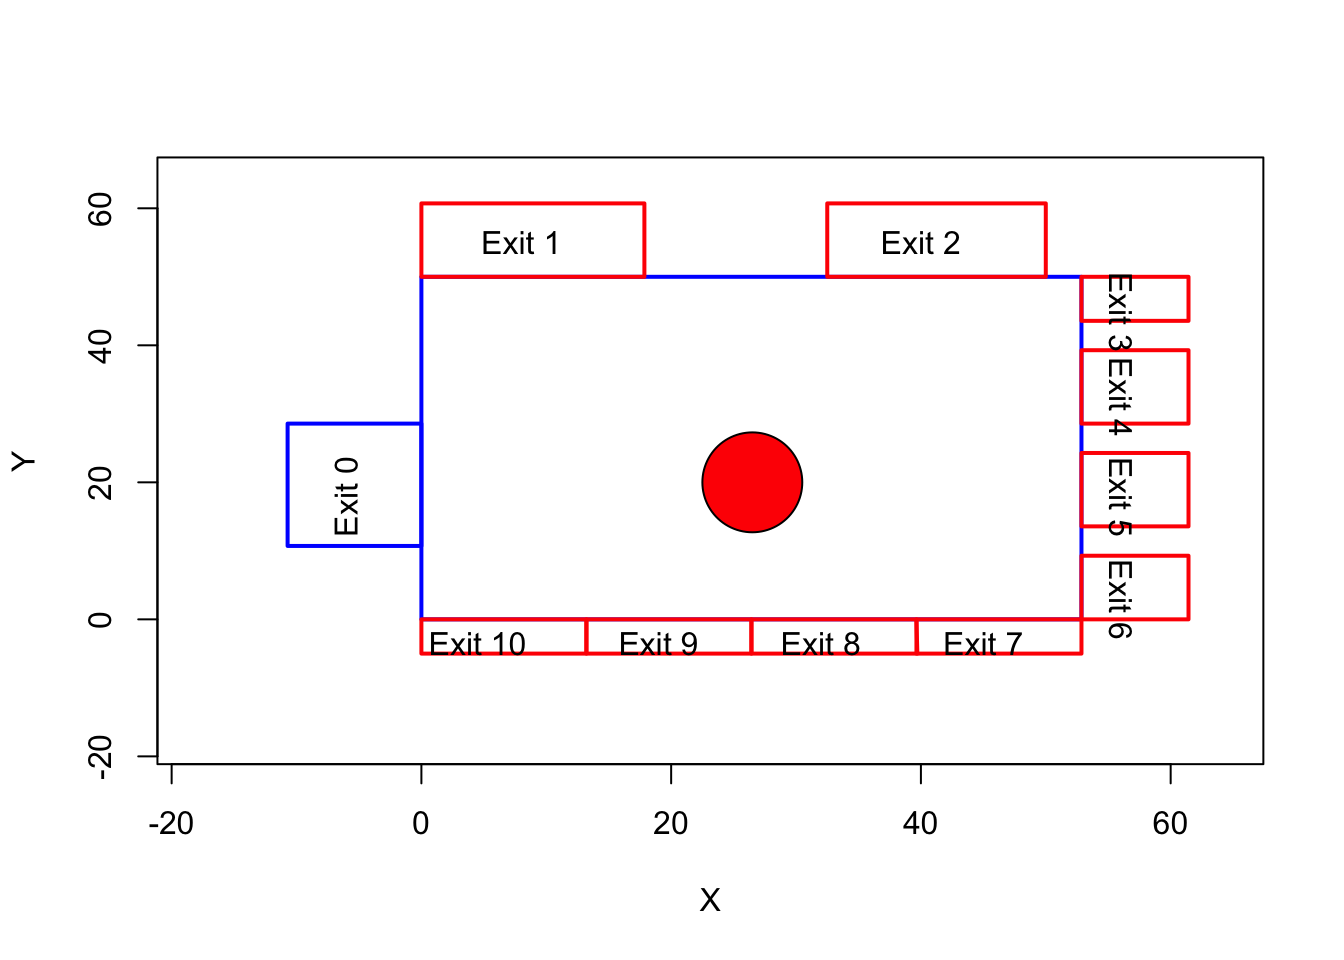
\includegraphics{./envir_files/figure-pdf/unnamed-chunk-1-1.pdf}

}

\end{figure}

\begin{Shaded}
\begin{Highlighting}[]
\CommentTok{\# now, let\textquotesingle{}s convert the env into an sf object}
\NormalTok{matrix\_walls }\OtherTok{=} \FunctionTok{matrix}\NormalTok{(}\FunctionTok{c}\NormalTok{(}\DecValTok{0}\NormalTok{,}\DecValTok{0}\NormalTok{,}\DecValTok{0}\NormalTok{,}\DecValTok{50}\NormalTok{,}\DecValTok{53}\NormalTok{,}\DecValTok{50}\NormalTok{, }\DecValTok{53}\NormalTok{,}\DecValTok{0}\NormalTok{,}\DecValTok{0}\NormalTok{,}\DecValTok{0}\NormalTok{),}
                      \AttributeTok{ncol =} \DecValTok{2}\NormalTok{,}
                      \AttributeTok{byrow =} \ConstantTok{TRUE}\NormalTok{)}
\NormalTok{matrixlist\_walls }\OtherTok{=} \FunctionTok{list}\NormalTok{(matrix\_walls)}
\NormalTok{polygon\_walls }\OtherTok{=}\NormalTok{ sf}\SpecialCharTok{::}\FunctionTok{st\_polygon}\NormalTok{(matrixlist\_walls)}

\CommentTok{\# calculate area size (will be needed for measuring density)}
\NormalTok{gcs\_area }\OtherTok{=}\NormalTok{ polygon\_walls }\SpecialCharTok{|\textgreater{}}\NormalTok{ sf}\SpecialCharTok{::}\FunctionTok{st\_area}\NormalTok{()}
\end{Highlighting}
\end{Shaded}

\hypertarget{divided}{%
\section{Divided}\label{divided}}

\begin{Shaded}
\begin{Highlighting}[]
\CommentTok{\# divide gcs polygon by creating a grid}
\NormalTok{gcs\_div }\OtherTok{=}\NormalTok{ sf}\SpecialCharTok{::}\FunctionTok{st\_make\_grid}\NormalTok{(polygon\_walls, }
                           \AttributeTok{n =} \DecValTok{2}\NormalTok{,}
                           \AttributeTok{what =} \StringTok{"polygons"}\NormalTok{)}

\CommentTok{\# convert gcs\_div to an sf object}
\NormalTok{gcs\_div\_sf }\OtherTok{=}\NormalTok{ gcs\_div }\SpecialCharTok{|\textgreater{}} 
\NormalTok{  sf}\SpecialCharTok{::}\FunctionTok{st\_as\_sf}\NormalTok{() }\SpecialCharTok{|\textgreater{}} 
\NormalTok{  dplyr}\SpecialCharTok{::}\FunctionTok{rename}\NormalTok{(}\AttributeTok{geom =}\NormalTok{ x)}

\CommentTok{\# find out the area size of each polygon}
\NormalTok{gcs\_area\_div }\OtherTok{=} \FunctionTok{list}\NormalTok{()}
\ControlFlowTok{for}\NormalTok{ (i }\ControlFlowTok{in} \DecValTok{1}\SpecialCharTok{:}\FunctionTok{lengths}\NormalTok{(gcs\_div\_sf))\{}
\NormalTok{  gcs\_area\_div[[i]] }\OtherTok{=}\NormalTok{ sf}\SpecialCharTok{::}\FunctionTok{st\_area}\NormalTok{(gcs\_div\_sf[[i]]) }
  \CommentTok{\# print(gcs\_area\_div)}
\NormalTok{\}}
\CommentTok{\# make it a vector}
\NormalTok{gcs\_area\_div }\OtherTok{=}\NormalTok{ gcs\_area\_div }\SpecialCharTok{|\textgreater{}}
  \FunctionTok{unlist}\NormalTok{() }\SpecialCharTok{|\textgreater{}}
  \FunctionTok{as.vector}\NormalTok{()}
\end{Highlighting}
\end{Shaded}

\hypertarget{selected}{%
\section{Selected}\label{selected}}

Two areas have been selected based on the results of the previous work:
https://github.com/Urban-Analytics/uncertainty/blob/master/gcs/process.ipynb
Hence, it's zone 1 (exit 0) and zone 2 (around exit 5) One cell is 2x2,
each zone is 5 (width) and 6 (length) cells, thus 10 and 12 metres
accordingly

Zone 1 is next to exit 0, thus its length has been left equal to the
length of the gates. The width has been approximated to 10 metres (1
pixel = 2 metres).

Zone 2 is on the opposite side to Zone 1 and is 1 pixel below comapred
to Zone 1, thus around exit 5.

\begin{Shaded}
\begin{Highlighting}[]
\DocumentationTok{\#\# zone 1 (it\textquotesingle{}s next to exit 0)}
\FunctionTok{gcs\_env\_m}\NormalTok{()}
\FunctionTok{polygon}\NormalTok{(}\AttributeTok{x =} \FunctionTok{c}\NormalTok{(}\DecValTok{10}\NormalTok{, }\DecValTok{0}\NormalTok{, }\DecValTok{0}\NormalTok{, }\DecValTok{10}\NormalTok{),}
        \AttributeTok{y =} \FunctionTok{c}\NormalTok{(}\DecValTok{28}\NormalTok{, }\DecValTok{28}\NormalTok{, }\DecValTok{10}\NormalTok{, }\DecValTok{10}\NormalTok{),}
        \AttributeTok{border =} \StringTok{"blue"}\NormalTok{,}
        \AttributeTok{lwd =} \DecValTok{2}\NormalTok{)}

\DocumentationTok{\#\# zone 2}
\CommentTok{\# gcs\_env\_m()}
\FunctionTok{polygon}\NormalTok{(}\AttributeTok{x =} \FunctionTok{c}\NormalTok{(}\DecValTok{53}\NormalTok{, }\DecValTok{43}\NormalTok{, }\DecValTok{43}\NormalTok{, }\DecValTok{53}\NormalTok{),}
        \AttributeTok{y =} \FunctionTok{c}\NormalTok{(}\DecValTok{26}\NormalTok{, }\DecValTok{26}\NormalTok{, }\DecValTok{8}\NormalTok{, }\DecValTok{8}\NormalTok{),}
        \AttributeTok{border =} \StringTok{"blue"}\NormalTok{,}
        \AttributeTok{lwd =} \DecValTok{2}\NormalTok{)}

\CommentTok{\# zone 1 sf polygon}
\NormalTok{zone1\_matrix }\OtherTok{=} \FunctionTok{matrix}\NormalTok{(}\FunctionTok{c}\NormalTok{(}\DecValTok{10}\NormalTok{, }\DecValTok{28}\NormalTok{, }\DecValTok{0}\NormalTok{, }\DecValTok{28}\NormalTok{, }\DecValTok{0}\NormalTok{, }\DecValTok{10}\NormalTok{, }\DecValTok{10}\NormalTok{, }\DecValTok{10}\NormalTok{, }\DecValTok{10}\NormalTok{, }\DecValTok{28}\NormalTok{),}
                      \AttributeTok{ncol =} \DecValTok{2}\NormalTok{,}
                      \AttributeTok{byrow =}\NormalTok{ T)}
\NormalTok{zone1\_matrix\_list }\OtherTok{=} \FunctionTok{list}\NormalTok{(zone1\_matrix)}
\NormalTok{zone1 }\OtherTok{=}\NormalTok{ sf}\SpecialCharTok{::}\FunctionTok{st\_polygon}\NormalTok{(zone1\_matrix\_list)}

\CommentTok{\# zone 2 sf polygon}
\NormalTok{zone2\_matrix }\OtherTok{=} \FunctionTok{matrix}\NormalTok{(}\FunctionTok{c}\NormalTok{(}\DecValTok{53}\NormalTok{, }\DecValTok{26}\NormalTok{, }\DecValTok{43}\NormalTok{, }\DecValTok{26}\NormalTok{, }\DecValTok{43}\NormalTok{, }\DecValTok{8}\NormalTok{, }\DecValTok{53}\NormalTok{, }\DecValTok{8}\NormalTok{, }\DecValTok{53}\NormalTok{, }\DecValTok{26}\NormalTok{),}
                      \AttributeTok{ncol =} \DecValTok{2}\NormalTok{,}
                      \AttributeTok{byrow =}\NormalTok{ T)}
\NormalTok{zone2\_matrix\_list }\OtherTok{=} \FunctionTok{list}\NormalTok{(zone2\_matrix)}
\NormalTok{zone2 }\OtherTok{=}\NormalTok{ sf}\SpecialCharTok{::}\FunctionTok{st\_polygon}\NormalTok{(zone2\_matrix\_list)}

\CommentTok{\# checking where selected areas are}
\FunctionTok{gcs\_env\_m}\NormalTok{()}
\NormalTok{zone1 }\SpecialCharTok{|\textgreater{}} \FunctionTok{plot}\NormalTok{(}\AttributeTok{add =}\NormalTok{ T, }\AttributeTok{border =} \StringTok{"green"}\NormalTok{, }\AttributeTok{lwd =} \DecValTok{2}\NormalTok{)}
\NormalTok{zone2 }\SpecialCharTok{|\textgreater{}} \FunctionTok{plot}\NormalTok{(}\AttributeTok{add =}\NormalTok{ T, }\AttributeTok{border =} \StringTok{"green"}\NormalTok{, }\AttributeTok{lwd =} \DecValTok{2}\NormalTok{)}

\CommentTok{\# join both zones}
\NormalTok{zones }\OtherTok{=} \FunctionTok{list}\NormalTok{(zone1, zone2)}
\end{Highlighting}
\end{Shaded}

\hypertarget{summary}{%
\chapter{Summary}\label{summary}}

In summary, this book has no content whatsoever.

\begin{Shaded}
\begin{Highlighting}[]
\DecValTok{1} \SpecialCharTok{+} \DecValTok{1}
\end{Highlighting}
\end{Shaded}

\begin{verbatim}
[1] 2
\end{verbatim}

\hypertarget{references}{%
\chapter*{References}\label{references}}
\addcontentsline{toc}{chapter}{References}

\hypertarget{refs}{}
\begin{CSLReferences}{0}{0}
\end{CSLReferences}



\end{document}
